\chapter{Related Work}\label{ch:related-work}

As the fields of \acrshort{vsn} \acrshort{rl} are very broad, this chapter aims to provide an extensive and organized overview of the most relevant works in the literature.
More specifically, this chapter delves into the main topics discussed alongside this thesis.
Since the main focus of this work is within robotic navigation, \acrlong{vsn} is the first topic covered.
It will lay the groundwork for how the other topics are related to robotic navigation and how they can be applied.
The following section will cover the sparsity and exploration methods, which are crucial for addressing the challenges of sparse rewards and exploration in \acrshort{rl}.
The next section will discuss the simulation-to-reality transfer in robotic navigation, which is essential for deploying models trained in simulation to real robots.
The subsequent section will cover offline \acrshort{rl}, which is a paradigm that allows training models using fixed datasets, without the need for online data collection.
Finally, the last section will discuss meta \acrshort{rl}, which focuses on learning policies that can quickly adapt to new environments.

While section~\ref{sec:visual-semantic-navigation} applies to the whole content of this document, the rest of the sections are more focused on the specific contributions of this thesis:

\begin{itemize}
    \item Section~\ref{sec:sparsity-and-exploration-methods} refers to chapter~\ref{ch:understanding-robotic-visual-semantic-navigation}, where we explore exploration methods based on the use of procedural environments and simulated environments.
    \item Section~\ref{sec:simulation-to-reality-transfer-in-robotic-navigation} is related to chapter~\ref{ch:ros4vsn:-enable-real-world-robotic-visual-semantic-navigation}, where we present the ROS4\acrshort{vsn} library, which allows the integration of different \acrshort{vsn} models in real robots.
    \item Section~\ref{sec:offline-reinforcement-learning} is related to chapter~\ref{sec:offline_rl4rvsn}, where we explore the use of offline \acrshort{rl} techniques to train navigation policies in simulated environments.
    \item Section~\ref{sec:meta-reinforcement-learning} is related to chapter~\ref{sec:mil-for-real-world-navigation}, where we explore the use of meta \acrshort{rl} techniques to train navigation policies that can quickly adapt to new environments.
\end{itemize}

\section{Visual Semantic Navigation}\label{sec:visual-semantic-navigation}

\acrfull{vsn} is a subfield of robotic navigation that focuses on enabling robots to navigate in environments using visual observations and semantic information.
In this context, semantic information refers to the understanding of the environment's objects and their relationships, which can be used to guide the robot's navigation decisions.
\acrshort{vsn} algorithms can be categorized into different approaches based on their training methods and architectures.
For the sake of clarity, this document follows the same categorization as~\cite{gervet2022}, depicted in figure~\ref{fig:vsn-categories}.

\begin{figure}
    \centering
    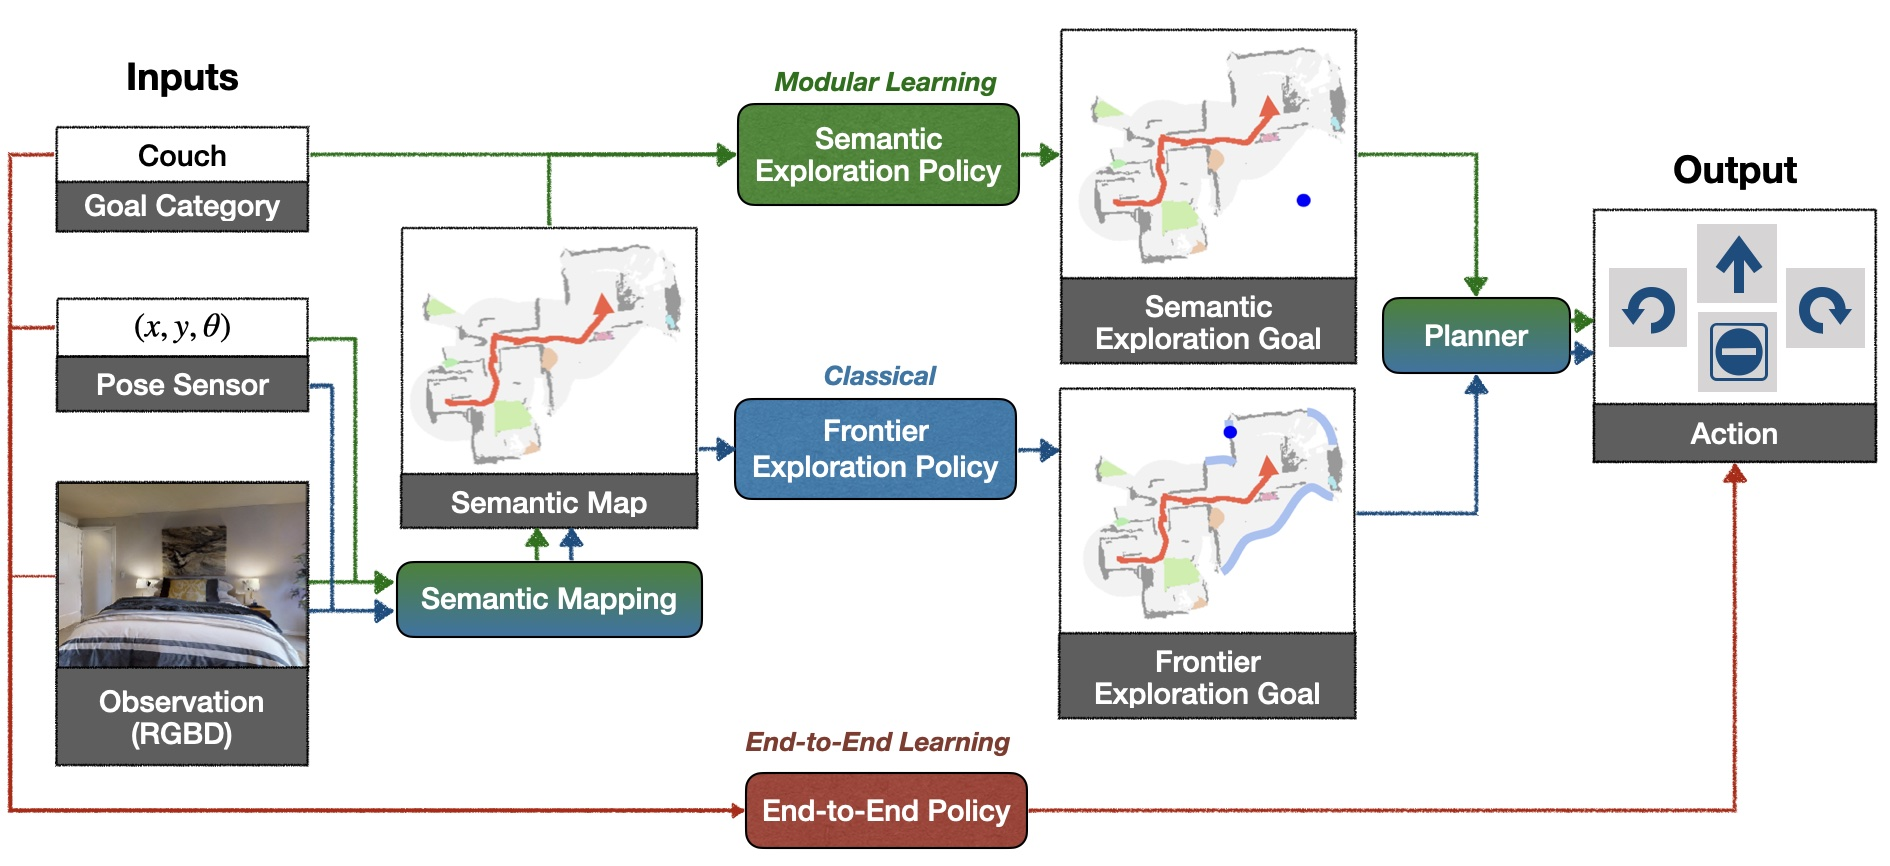
\includegraphics[width=\textwidth]{figures/related_work/methods_overview}
    \caption{Categories of visual semantic navigation approaches.}
    \label{fig:vsn-categories}
\end{figure}

To navigate in unfamiliar environments, traditional methods use depth sensors~\cite{newcombe2011, thrun2001} and RGB cameras~\cite{jones2011, sattler2018} to build geometric maps and simultaneously determine the robot's position in relation to the map.
This is known as Simultaneous Localization and Mapping (SLAM)~\cite{Kazerouni2022, campos2021, labbe2022}).
Typically, these SLAM models use heuristic algorithms to create graph-based representations of the environment, allowing the robot to visit the different nodes of the graph when navigating to specific points.
Semantic SLAM (\eg~\cite{zhang2018, rosinol2020, jin2023}) expands upon SLAM by integrating semantic data from the environment, allowing the robot to identify and store objects in memory.

A recent approach, made possible by advances in machine learning and computer vision, involves designing navigation policies that directly train deep neural networks to learn semantic information from visual observations in an end-to-end fashion (\eg~\cite{ramrakhya2022,yadav2022, gutierrez2019, khandelwal2022, chaplot2020,chang2020}).
This approach is termed \textit{visual semantic navigation} (\acrshort{vsn}).
These models often rely on the use of CNNs as visual encoders followed by RNNs; that are in charge of predicting an action distribution directly from raw input observations.
The neural networks are trained using imitation learning (IL) or reinforcement learning (RL) approaches.

When IL is applied to the visual navigation problem, navigation policies are learnt from expert demonstrations (\eg~\cite{ramrakhya2022,yadav2022}).
It can also be used combined with an RL fine-tuning phase to achieve better performance~\cite{ramrakhya2023}.

Other works focus on the use of an end-to-end RL approach to solve \objnav navigation~\cite{zhu2017, gutierrez2019, wijmans2020, khandelwal2022, Liu2022, Yadav2023OVRLV2AS, Xu2024DeepRL, YokoyamaHM3DOVONAD}.
Some authors have proposed combining the RL training with different strategies, like auxiliary tasks~\cite{ye2021}, improved visual representations via object relation graphs~\cite{yang2018}, semantic segmentations~\cite{Mousavian2018} or combining audio feedback with the visual inputs~\cite{Wang2023, Kondoh2023MultigoalAN}.

Modular-learning based approaches~\cite{chaplot2020, chang2020, skillfusion, Li2023RDDRLAR, zhou2022improving, Cai2024DGMemLV, Kang2024HSPNavHS, Wang2023ProbableOL, Wasserman2023ExploitationGuidedEF, Yokoyama2023VLFMVF} decompose the navigation process in separate modules that execute different tasks.
It is common for these methods to be composed of a high-level semantic exploration module trained by RL that indicates the agent subgoals that have to be reached by a low-level navigation policy.
Modular learning can be also combined with offline RL~\cite{shah2022} techniques to leverage navigation behaviors from fixed datasets, without any additional online data collection or fine-tuning.

Finally, there are different approaches that try to tackle the problem of rapidly adapting to unseen environments in visual navigation via meta-learning~\cite{wortsman2019, luo2021, zhang2022}.
These methods are trained on a variety of different environments (usually designated as tasks) and are able to generalize to unseen environments by learning a policy that can be quickly adapted to new environments.
And the recent progress in large language models (LLMs) has led to the possibility of using them to solve the visual navigation problem~\cite{Huang2023, Zhou2023} as well.
In this case, the LLMs are used as a reasoning module in charge of understanding the semantic information present on the environment.
They then share this information with different modules in charge of navigating to the specified goal.

Our goal in this work is not to develope \acrshort{vsn} approaches, but to integrate various state-of-the-art \acrshort{vsn} models into multiple real-world robots by using our novel ROS4\acrshort{vsn} library.
Technically, we have chosen to integrate the PIRLNav~\cite{ramrakhya2023} and VLV~\cite{chang2020} models into two different robots.
These integrations required several technical adaptations, particularly in the areas of sensor data integration and navigation planning.
Overall, we are able to show how ROS4\acrshort{vsn} allows easily testing and comparing different \acrshort{vsn} methods in the real world.
To the best of our knowledge, our work is the first to develop a model agnostic ROS package for visual semantic navigation, where multiple models can be integrated.

\section{Sparsity and exploration methods}\label{sec:sparsity-and-exploration-methods}
To address the sparse reward and exploration problems, different approaches have been proposed.
Auxiliary tasks~\cite{jaderberg2016, ye2021} help the agent to explore the environment and gather extrinsic reward by maximizing pseudo-reward functions.
Curiosity-driven exploration~\cite{pathak2017} leverages on the error of the agent's ability to predict the next state to introduce a new intrinsic reward that enables the agent to explore the environment.
When dealing with procedurally-generated environments, a curriculum learning mechanism can be incorporated so the episodes are ordered by an exploration score~\cite{zha2020b}, and then the agent imitates the best ones.
We also use procedurally-generated environments, but we rely on a RL approach combined with reward shaping~\cite{ng1999, jestel2021} and $\epsilon\text{-}greedy$~\cite{mnih2013} techniques to learn to navigate in them.

\section{Simulation-to-reality transfer in robotic navigation}\label{sec:simulation-to-reality-transfer-in-robotic-navigation}
Deploying a model trained in simulation to a real robot is a challenging task.
Due to logistical constraints, training a model in the real world —especially with RL techniques— is often impractical, prompting the use of alternative methods to address this challenge
For example, \cite{kim2022} propose a monocular vision-based time-to-collision estimation for small drones by domain adaptation of simulated images.
Their method converts simulated images into real-like synthetic images using a sim-to-real method.
This is done with the aim of minimizing efforts and time invested in the collection of training datasets within real-world scenarios, while simultaneously maximizing the advantages inherent in simulated environments.

Overall, it is necessary to develop methods that allow to efficiently transfer the knowledge learnt in simulation to the real world~\cite{kadian2020}.
Different approaches have been proposed to solve this problem.
For instance, CAD2RL~\cite{sadeghiCAD2RLRealSingleImage2017} system achieved remarkable success in training a collision avoidance policy entirely within a simulated environment.
This breakthrough was subsequently tested on real aerial drones, with promising results.
By focusing on simulation refinement~\cite{Son2020}, the accuracy of simulations can be improved by exploiting the disparities between simulated and real-world observations.
In the field of locomotion, training legged robotic systems in a simulated environment and subsequently transferring the acquired policies to real-world applications~\cite{Hwangbo_2019, agarwal2022} has always been a challenging task.

For the problem of \acrshort{vsn}, we have the studiy by \cite{gervet2022} that shows how their approaches perform in real-world settings.
However, we would like to highlight the novel contributions that our work offers.
First, while~\cite{gervet2022} focuses mainly on the comparison of their navigation methods, we here, along with a similar study, release to the research community the modular ROS4\acrshort{vsn} software architecture.
Our main goal is to facilitate the prototyping of new \acrshort{vsn} solutions on real robots.
So, we offer a ROS-compatible software architecture, model agnostic, that allows a simple integration of different \acrshort{vsn} approaches in ROS robots.
In this way, future \acrshort{vsn} solutions will be able to be tested on real robots in a convenient and straightforward manner.
Second, we include in our study more recent \acrshort{vsn} solutions than the ones reported in~\cite{gervet2022}, as the PIRLNav model~\cite{ramrakhya2023}, which defines the state-of-the-art for the \objnav problem.
Third, we also provide, for the first time, a detailed analysis on how a model directly trained with real videos, such as the VLV~\cite{chang2020}, performs in real robots.
This allows us to compare, as in~\cite{gervet2022}, how a modular-learning model (\ie VLV~\cite{chang2020}), compares with a typical end-to-end learning approach (\ie PIRLNav).
Interestingly, our study also concludes, like in~\cite{gervet2022}, that modular-learning approaches perform better in the real world.
Fourth, in our study, we employed two different robotic platforms: one commercially available and widely used by various laboratories, and another custom-built.
This demonstrates the versatility of the proposed solution, showing that it can be integrated into different robots.
And finally, in our work, we propose an experimental evaluation specifically designed for testing in the real world, which can be employed in future research studies.
Overall, we hope that our ROS-based library will help to further advance the field of visual semantic navigation in real robots.

\section{Offline Reinforcement Learning}\label{sec:offline-reinforcement-learning}

\section{Meta Reinforcement Learning}\label{sec:meta-reinforcement-learning}